% Options for packages loaded elsewhere
\PassOptionsToPackage{unicode}{hyperref}
\PassOptionsToPackage{hyphens}{url}
%
\documentclass[
]{article}
\usepackage{amsmath,amssymb}
\usepackage{lmodern}
\usepackage{iftex}
\ifPDFTeX
  \usepackage[T1]{fontenc}
  \usepackage[utf8]{inputenc}
  \usepackage{textcomp} % provide euro and other symbols
\else % if luatex or xetex
  \usepackage{unicode-math}
  \defaultfontfeatures{Scale=MatchLowercase}
  \defaultfontfeatures[\rmfamily]{Ligatures=TeX,Scale=1}
\fi
% Use upquote if available, for straight quotes in verbatim environments
\IfFileExists{upquote.sty}{\usepackage{upquote}}{}
\IfFileExists{microtype.sty}{% use microtype if available
  \usepackage[]{microtype}
  \UseMicrotypeSet[protrusion]{basicmath} % disable protrusion for tt fonts
}{}
\makeatletter
\@ifundefined{KOMAClassName}{% if non-KOMA class
  \IfFileExists{parskip.sty}{%
    \usepackage{parskip}
  }{% else
    \setlength{\parindent}{0pt}
    \setlength{\parskip}{6pt plus 2pt minus 1pt}}
}{% if KOMA class
  \KOMAoptions{parskip=half}}
\makeatother
\usepackage{xcolor}
\usepackage[margin=1in]{geometry}
\usepackage{color}
\usepackage{fancyvrb}
\newcommand{\VerbBar}{|}
\newcommand{\VERB}{\Verb[commandchars=\\\{\}]}
\DefineVerbatimEnvironment{Highlighting}{Verbatim}{commandchars=\\\{\}}
% Add ',fontsize=\small' for more characters per line
\usepackage{framed}
\definecolor{shadecolor}{RGB}{248,248,248}
\newenvironment{Shaded}{\begin{snugshade}}{\end{snugshade}}
\newcommand{\AlertTok}[1]{\textcolor[rgb]{0.94,0.16,0.16}{#1}}
\newcommand{\AnnotationTok}[1]{\textcolor[rgb]{0.56,0.35,0.01}{\textbf{\textit{#1}}}}
\newcommand{\AttributeTok}[1]{\textcolor[rgb]{0.77,0.63,0.00}{#1}}
\newcommand{\BaseNTok}[1]{\textcolor[rgb]{0.00,0.00,0.81}{#1}}
\newcommand{\BuiltInTok}[1]{#1}
\newcommand{\CharTok}[1]{\textcolor[rgb]{0.31,0.60,0.02}{#1}}
\newcommand{\CommentTok}[1]{\textcolor[rgb]{0.56,0.35,0.01}{\textit{#1}}}
\newcommand{\CommentVarTok}[1]{\textcolor[rgb]{0.56,0.35,0.01}{\textbf{\textit{#1}}}}
\newcommand{\ConstantTok}[1]{\textcolor[rgb]{0.00,0.00,0.00}{#1}}
\newcommand{\ControlFlowTok}[1]{\textcolor[rgb]{0.13,0.29,0.53}{\textbf{#1}}}
\newcommand{\DataTypeTok}[1]{\textcolor[rgb]{0.13,0.29,0.53}{#1}}
\newcommand{\DecValTok}[1]{\textcolor[rgb]{0.00,0.00,0.81}{#1}}
\newcommand{\DocumentationTok}[1]{\textcolor[rgb]{0.56,0.35,0.01}{\textbf{\textit{#1}}}}
\newcommand{\ErrorTok}[1]{\textcolor[rgb]{0.64,0.00,0.00}{\textbf{#1}}}
\newcommand{\ExtensionTok}[1]{#1}
\newcommand{\FloatTok}[1]{\textcolor[rgb]{0.00,0.00,0.81}{#1}}
\newcommand{\FunctionTok}[1]{\textcolor[rgb]{0.00,0.00,0.00}{#1}}
\newcommand{\ImportTok}[1]{#1}
\newcommand{\InformationTok}[1]{\textcolor[rgb]{0.56,0.35,0.01}{\textbf{\textit{#1}}}}
\newcommand{\KeywordTok}[1]{\textcolor[rgb]{0.13,0.29,0.53}{\textbf{#1}}}
\newcommand{\NormalTok}[1]{#1}
\newcommand{\OperatorTok}[1]{\textcolor[rgb]{0.81,0.36,0.00}{\textbf{#1}}}
\newcommand{\OtherTok}[1]{\textcolor[rgb]{0.56,0.35,0.01}{#1}}
\newcommand{\PreprocessorTok}[1]{\textcolor[rgb]{0.56,0.35,0.01}{\textit{#1}}}
\newcommand{\RegionMarkerTok}[1]{#1}
\newcommand{\SpecialCharTok}[1]{\textcolor[rgb]{0.00,0.00,0.00}{#1}}
\newcommand{\SpecialStringTok}[1]{\textcolor[rgb]{0.31,0.60,0.02}{#1}}
\newcommand{\StringTok}[1]{\textcolor[rgb]{0.31,0.60,0.02}{#1}}
\newcommand{\VariableTok}[1]{\textcolor[rgb]{0.00,0.00,0.00}{#1}}
\newcommand{\VerbatimStringTok}[1]{\textcolor[rgb]{0.31,0.60,0.02}{#1}}
\newcommand{\WarningTok}[1]{\textcolor[rgb]{0.56,0.35,0.01}{\textbf{\textit{#1}}}}
\usepackage{graphicx}
\makeatletter
\def\maxwidth{\ifdim\Gin@nat@width>\linewidth\linewidth\else\Gin@nat@width\fi}
\def\maxheight{\ifdim\Gin@nat@height>\textheight\textheight\else\Gin@nat@height\fi}
\makeatother
% Scale images if necessary, so that they will not overflow the page
% margins by default, and it is still possible to overwrite the defaults
% using explicit options in \includegraphics[width, height, ...]{}
\setkeys{Gin}{width=\maxwidth,height=\maxheight,keepaspectratio}
% Set default figure placement to htbp
\makeatletter
\def\fps@figure{htbp}
\makeatother
\setlength{\emergencystretch}{3em} % prevent overfull lines
\providecommand{\tightlist}{%
  \setlength{\itemsep}{0pt}\setlength{\parskip}{0pt}}
\setcounter{secnumdepth}{-\maxdimen} % remove section numbering
\ifLuaTeX
  \usepackage{selnolig}  % disable illegal ligatures
\fi
\IfFileExists{bookmark.sty}{\usepackage{bookmark}}{\usepackage{hyperref}}
\IfFileExists{xurl.sty}{\usepackage{xurl}}{} % add URL line breaks if available
\urlstyle{same} % disable monospaced font for URLs
\hypersetup{
  pdftitle={HW5},
  hidelinks,
  pdfcreator={LaTeX via pandoc}}

\title{HW5}
\author{}
\date{\vspace{-2.5em}2023-03-31}

\begin{document}
\maketitle

\hypertarget{question-1}{%
\subsubsection{QUESTION 1}\label{question-1}}

\hypertarget{a-model-fitting-and-interpretation}{%
\paragraph{(a) Model Fitting and
Interpretation}\label{a-model-fitting-and-interpretation}}

\begin{Shaded}
\begin{Highlighting}[]
\DocumentationTok{\#\# fit a poisson log{-}link model}
\NormalTok{crab }\OtherTok{=} \FunctionTok{read.table}\NormalTok{(}\StringTok{"HW5{-}crab.txt"}\NormalTok{, }\AttributeTok{header =} \ConstantTok{TRUE}\NormalTok{)}
\NormalTok{M1 }\OtherTok{=} \FunctionTok{glm}\NormalTok{(Sa }\SpecialCharTok{\textasciitilde{}}\NormalTok{ W, }\AttributeTok{family=}\FunctionTok{poisson}\NormalTok{(}\AttributeTok{link=}\NormalTok{log), }\AttributeTok{data=}\NormalTok{crab)}
\FunctionTok{summary}\NormalTok{(M1)}
\end{Highlighting}
\end{Shaded}

\begin{verbatim}
## 
## Call:
## glm(formula = Sa ~ W, family = poisson(link = log), data = crab)
## 
## Deviance Residuals: 
##     Min       1Q   Median       3Q      Max  
## -2.8526  -1.9884  -0.4933   1.0970   4.9221  
## 
## Coefficients:
##             Estimate Std. Error z value Pr(>|z|)    
## (Intercept) -3.30476    0.54224  -6.095  1.1e-09 ***
## W            0.16405    0.01997   8.216  < 2e-16 ***
## ---
## Signif. codes:  0 '***' 0.001 '**' 0.01 '*' 0.05 '.' 0.1 ' ' 1
## 
## (Dispersion parameter for poisson family taken to be 1)
## 
##     Null deviance: 632.79  on 172  degrees of freedom
## Residual deviance: 567.88  on 171  degrees of freedom
## AIC: 927.18
## 
## Number of Fisher Scoring iterations: 6
\end{verbatim}

\begin{Shaded}
\begin{Highlighting}[]
\CommentTok{\# goodness of fit}
\NormalTok{res.pearson }\OtherTok{=} \FunctionTok{residuals}\NormalTok{(M1, }\AttributeTok{type=}\StringTok{"pearson"}\NormalTok{)}
\NormalTok{G.stat }\OtherTok{=} \FunctionTok{sum}\NormalTok{(res.pearson}\SpecialCharTok{\^{}}\DecValTok{2}\NormalTok{)}
\NormalTok{res.dev }\OtherTok{=} \FunctionTok{residuals}\NormalTok{(M1, }\AttributeTok{type=}\StringTok{"deviance"}\NormalTok{)}
\NormalTok{D.stat }\OtherTok{=} \FunctionTok{sum}\NormalTok{(res.dev}\SpecialCharTok{\^{}}\DecValTok{2}\NormalTok{)}
\DecValTok{1}\SpecialCharTok{{-}}\FunctionTok{pchisq}\NormalTok{(G.stat, }\AttributeTok{df=}\DecValTok{173{-}2}\NormalTok{)}
\end{Highlighting}
\end{Shaded}

\begin{verbatim}
## [1] 0
\end{verbatim}

\begin{Shaded}
\begin{Highlighting}[]
\DecValTok{1}\SpecialCharTok{{-}}\FunctionTok{pchisq}\NormalTok{(D.stat, }\AttributeTok{df=}\DecValTok{173{-}2}\NormalTok{)}
\end{Highlighting}
\end{Shaded}

\begin{verbatim}
## [1] 0
\end{verbatim}

\textbf{Goodness of fit:}

The Pearson's Chi-square test statistic is 544.16, deviance test
statistic is 567.88. The p-values of both of them are less than 0.05
under 171 df, indicating the fit is not good here.

\textbf{Interpretation of the model:}

We fitted a poisson log linear model here where:

log(E(Y)) = β0 + β1·X

with Y=Sa (number of satellites), X=W (carapace width).

Here β0 = -3.3, β1 = 0.16. Indicating that when the carapace width is 0,
the expected number of satellites is 0.04 . When there's one unit change
in carapace width, the expected change in the number of satellites is
1.18.

\hypertarget{b-model-fitting-with-more-predictors-and-interpretation}{%
\paragraph{(b) Model Fitting with More Predictors and
Interpretation}\label{b-model-fitting-with-more-predictors-and-interpretation}}

\begin{Shaded}
\begin{Highlighting}[]
\CommentTok{\# fit again with 2 predictors}
\NormalTok{M2 }\OtherTok{=} \FunctionTok{glm}\NormalTok{(Sa }\SpecialCharTok{\textasciitilde{}}\NormalTok{ W }\SpecialCharTok{+}\NormalTok{ Wt, }\AttributeTok{family=}\FunctionTok{poisson}\NormalTok{(}\AttributeTok{link=}\NormalTok{log), }\AttributeTok{data=}\NormalTok{crab)}
\FunctionTok{summary}\NormalTok{(M2)}
\end{Highlighting}
\end{Shaded}

\begin{verbatim}
## 
## Call:
## glm(formula = Sa ~ W + Wt, family = poisson(link = log), data = crab)
## 
## Deviance Residuals: 
##     Min       1Q   Median       3Q      Max  
## -2.9308  -1.9705  -0.5481   0.9700   4.9905  
## 
## Coefficients:
##             Estimate Std. Error z value Pr(>|z|)   
## (Intercept) -1.29168    0.89929  -1.436  0.15091   
## W            0.04590    0.04677   0.981  0.32640   
## Wt           0.44744    0.15864   2.820  0.00479 **
## ---
## Signif. codes:  0 '***' 0.001 '**' 0.01 '*' 0.05 '.' 0.1 ' ' 1
## 
## (Dispersion parameter for poisson family taken to be 1)
## 
##     Null deviance: 632.79  on 172  degrees of freedom
## Residual deviance: 559.89  on 170  degrees of freedom
## AIC: 921.18
## 
## Number of Fisher Scoring iterations: 6
\end{verbatim}

\begin{Shaded}
\begin{Highlighting}[]
\CommentTok{\# goodness of fit}
\NormalTok{res.pearson2 }\OtherTok{=} \FunctionTok{residuals}\NormalTok{(M2, }\AttributeTok{type=}\StringTok{"pearson"}\NormalTok{)}
\NormalTok{G.stat2 }\OtherTok{=} \FunctionTok{sum}\NormalTok{(res.pearson2}\SpecialCharTok{\^{}}\DecValTok{2}\NormalTok{)}
\NormalTok{res.dev2 }\OtherTok{=} \FunctionTok{residuals}\NormalTok{(M2, }\AttributeTok{type=}\StringTok{"deviance"}\NormalTok{)}
\NormalTok{D.stat2 }\OtherTok{=} \FunctionTok{sum}\NormalTok{(res.dev2}\SpecialCharTok{\^{}}\DecValTok{2}\NormalTok{)}
\DecValTok{1}\SpecialCharTok{{-}}\FunctionTok{pchisq}\NormalTok{(G.stat2, }\AttributeTok{df=}\DecValTok{173{-}3}\NormalTok{)}
\end{Highlighting}
\end{Shaded}

\begin{verbatim}
## [1] 0
\end{verbatim}

\begin{Shaded}
\begin{Highlighting}[]
\DecValTok{1}\SpecialCharTok{{-}}\FunctionTok{pchisq}\NormalTok{(D.stat2, }\AttributeTok{df=}\DecValTok{173{-}3}\NormalTok{)}
\end{Highlighting}
\end{Shaded}

\begin{verbatim}
## [1] 0
\end{verbatim}

\begin{Shaded}
\begin{Highlighting}[]
\CommentTok{\# compare 2 models}
\NormalTok{test.stat }\OtherTok{=}\NormalTok{ M1}\SpecialCharTok{$}\NormalTok{deviance }\SpecialCharTok{{-}}\NormalTok{ M2}\SpecialCharTok{$}\NormalTok{deviance}
\NormalTok{df }\OtherTok{=} \DecValTok{171{-}170}
\NormalTok{pv3 }\OtherTok{=}  \DecValTok{1}\SpecialCharTok{{-}}\FunctionTok{pchisq}\NormalTok{(test.stat, }\AttributeTok{df =}\NormalTok{ df)}
\NormalTok{pv3 }\CommentTok{\# rej, choose larger model}
\end{Highlighting}
\end{Shaded}

\begin{verbatim}
## [1] 0.004694838
\end{verbatim}

The Pearson's Chi-square test statistic is 536.6, deviance test
statistic is 559.89. The p-values of both of them are less than 0.05
under 170 df, indicating the fit is not good here. However, the p-value
of the deviance test comparing the two models is less than 0.05 under 1
df, indicating that we should choose the larger model over the smaller
one.

\hypertarget{c-overdispersion-adjustment}{%
\paragraph{(c) Overdispersion
Adjustment}\label{c-overdispersion-adjustment}}

\begin{Shaded}
\begin{Highlighting}[]
\CommentTok{\# plot half{-}normal plot}
\NormalTok{abs\_res }\OtherTok{=} \FunctionTok{abs}\NormalTok{(res.pearson2)}
\FunctionTok{plot}\NormalTok{(}\FunctionTok{qnorm}\NormalTok{((}\DecValTok{173}\SpecialCharTok{+}\DecValTok{1}\SpecialCharTok{:}\DecValTok{173}\FloatTok{+0.5}\NormalTok{)}\SpecialCharTok{/}\NormalTok{(}\DecValTok{2}\SpecialCharTok{*}\DecValTok{173}\FloatTok{+1.125}\NormalTok{)),}\FunctionTok{sort}\NormalTok{(abs\_res))}
\FunctionTok{abline}\NormalTok{(}\AttributeTok{a=}\DecValTok{0}\NormalTok{,}\AttributeTok{b=}\DecValTok{1}\NormalTok{)}
\end{Highlighting}
\end{Shaded}

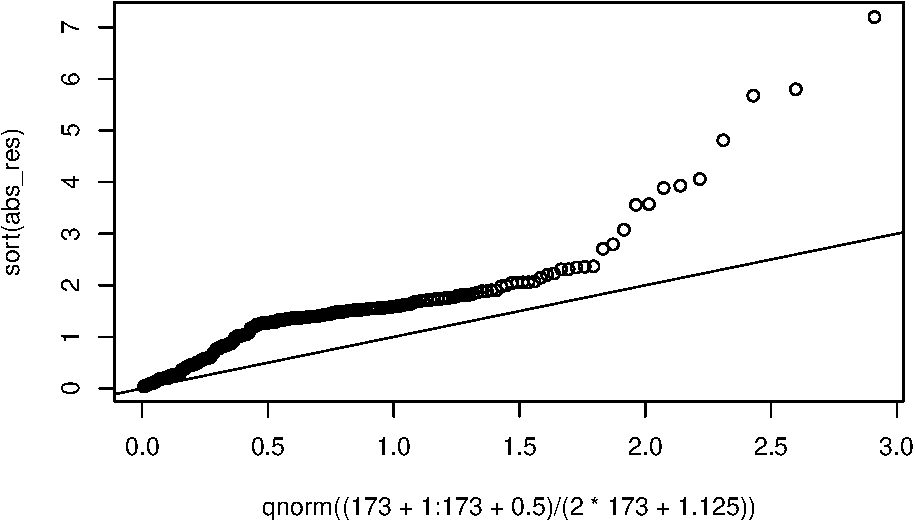
\includegraphics{HW5_files/figure-latex/unnamed-chunk-4-1.pdf}

\begin{Shaded}
\begin{Highlighting}[]
\CommentTok{\# estimate dispersion parameter}
\NormalTok{res.p1 }\OtherTok{=} \FunctionTok{residuals}\NormalTok{(M2, }\AttributeTok{type=}\StringTok{\textquotesingle{}pearson\textquotesingle{}}\NormalTok{, }\AttributeTok{data=}\NormalTok{crab)}
\NormalTok{G1 }\OtherTok{=} \FunctionTok{sum}\NormalTok{(res.p1}\SpecialCharTok{\^{}}\DecValTok{2}\NormalTok{)}
\NormalTok{phi }\OtherTok{=}\NormalTok{ G1}\SpecialCharTok{/}\NormalTok{(}\DecValTok{173{-}3}\NormalTok{)}
\NormalTok{phi}
\end{Highlighting}
\end{Shaded}

\begin{verbatim}
## [1] 3.156449
\end{verbatim}

\begin{Shaded}
\begin{Highlighting}[]
\CommentTok{\# refit with phi}
\FunctionTok{summary}\NormalTok{(M2, }\AttributeTok{dispersion=}\NormalTok{phi)}
\end{Highlighting}
\end{Shaded}

\begin{verbatim}
## 
## Call:
## glm(formula = Sa ~ W + Wt, family = poisson(link = log), data = crab)
## 
## Deviance Residuals: 
##     Min       1Q   Median       3Q      Max  
## -2.9308  -1.9705  -0.5481   0.9700   4.9905  
## 
## Coefficients:
##             Estimate Std. Error z value Pr(>|z|)
## (Intercept) -1.29168    1.59771  -0.808    0.419
## W            0.04590    0.08309   0.552    0.581
## Wt           0.44744    0.28184   1.588    0.112
## 
## (Dispersion parameter for poisson family taken to be 3.156449)
## 
##     Null deviance: 632.79  on 172  degrees of freedom
## Residual deviance: 559.89  on 170  degrees of freedom
## AIC: 921.18
## 
## Number of Fisher Scoring iterations: 6
\end{verbatim}

\begin{Shaded}
\begin{Highlighting}[]
\CommentTok{\# goodness of fit}
\NormalTok{pv.od }\OtherTok{=} \DecValTok{1}\SpecialCharTok{{-}}\FunctionTok{pchisq}\NormalTok{(}\DecValTok{173{-}3}\NormalTok{, }\AttributeTok{df=}\DecValTok{173{-}3}\NormalTok{)}
\end{Highlighting}
\end{Shaded}

The dispersion parameter is 3.16 in M2. There is a deviation from the
reference line with slope 1, indicating constant over-dispersion. After
adjusting for dispersion=3.16, the model parameters are the same as
before, but the p-value for the Chi-square test is 0.49 here, greater
than 0.05, indicating a good fit.

\hypertarget{question-2}{%
\subsubsection{QUESTION 2}\label{question-2}}

\hypertarget{a-model-fitting-and-interpretation-1}{%
\paragraph{(a) Model Fitting and
Interpretation}\label{a-model-fitting-and-interpretation-1}}

\begin{Shaded}
\begin{Highlighting}[]
\CommentTok{\# fit a poisson log{-}link model}
\NormalTok{fish }\OtherTok{=} \FunctionTok{read.table}\NormalTok{(}\StringTok{"HW5{-}parasite.txt"}\NormalTok{, }\AttributeTok{header =} \ConstantTok{TRUE}\NormalTok{)}
\NormalTok{fish }\OtherTok{=} 
\NormalTok{  fish }\SpecialCharTok{\%\textgreater{}\%} 
  \FunctionTok{mutate}\NormalTok{(}\AttributeTok{Area =} \FunctionTok{as.factor}\NormalTok{(Area),}
         \AttributeTok{Year =} \FunctionTok{as.factor}\NormalTok{(Year)) }
\NormalTok{M1.fish }\OtherTok{=} \FunctionTok{glm}\NormalTok{(Intensity }\SpecialCharTok{\textasciitilde{}}\NormalTok{ Area }\SpecialCharTok{+}\NormalTok{ Year }\SpecialCharTok{+}\NormalTok{ Length, }\AttributeTok{family=}\FunctionTok{poisson}\NormalTok{(}\AttributeTok{link=}\NormalTok{log), }\AttributeTok{data=}\NormalTok{fish)}
\FunctionTok{summary}\NormalTok{(M1.fish)}
\end{Highlighting}
\end{Shaded}

\begin{verbatim}
## 
## Call:
## glm(formula = Intensity ~ Area + Year + Length, family = poisson(link = log), 
##     data = fish)
## 
## Deviance Residuals: 
##     Min       1Q   Median       3Q      Max  
## -9.3632  -2.7158  -2.0142  -0.4731  30.2492  
## 
## Coefficients:
##               Estimate Std. Error z value Pr(>|z|)    
## (Intercept)  2.6431709  0.0542838  48.692  < 2e-16 ***
## Area2       -0.2119557  0.0491691  -4.311 1.63e-05 ***
## Area3       -0.1168602  0.0428296  -2.728  0.00636 ** 
## Area4        1.4049366  0.0356625  39.395  < 2e-16 ***
## Year2000     0.6702801  0.0279823  23.954  < 2e-16 ***
## Year2001    -0.2181393  0.0287535  -7.587 3.29e-14 ***
## Length      -0.0284228  0.0008809 -32.265  < 2e-16 ***
## ---
## Signif. codes:  0 '***' 0.001 '**' 0.01 '*' 0.05 '.' 0.1 ' ' 1
## 
## (Dispersion parameter for poisson family taken to be 1)
## 
##     Null deviance: 25797  on 1190  degrees of freedom
## Residual deviance: 19153  on 1184  degrees of freedom
##   (63 observations deleted due to missingness)
## AIC: 21089
## 
## Number of Fisher Scoring iterations: 7
\end{verbatim}

\textbf{Interpretation of the model:}

We fitted a poisson log linear model here where:

log(E(Y)) = β0 + β1·X1 + β2·X2 + β3·X3

with Y = Intensity, X1 = Area2, X2 = Area3, X3 = Area3, X4 = Year2000,
X5 = Year2001, X5 = Length.

\begin{itemize}
\item
  Here exp(β1) = 0.81, indicating that adjusting for year and length,
  the expected intensity of parasite in area2 is 0.81 times of that in
  area1.
\item
  exp(β2) = 0.89, indicating that adjusting for year and length, the
  expected intensity of parasite in area3 is 0.89 times of that in
  area1.
\item
  exp(β3) = 4.08, indicating that adjusting for year and length, the
  expected intensity of parasite in area4 is 4.08 times of that in
  area1.
\item
  exp(β4) = 1.95, indicating that adjusting for area and length, the
  expected intensity of parasite in year 2000 is 1.95 times of that in
  year 1999.
\item
  exp(β5) = 0.8, indicating that adjusting for area and length, the
  expected intensity of parasite in year 2001 is 0.8 times of that in
  year 1999.
\item
  exp(β6) = 0.97, indicating that adjusting for area and year, with one
  unit increase in length, the expected intensity of parasite would
  decrease by 0.97 times.
\end{itemize}

\hypertarget{b-goodness-of-fit}{%
\paragraph{(b) Goodness of Fit}\label{b-goodness-of-fit}}

\begin{Shaded}
\begin{Highlighting}[]
\CommentTok{\# goodness of fit}
\NormalTok{res.pearson.fish }\OtherTok{=} \FunctionTok{residuals}\NormalTok{(M1.fish, }\AttributeTok{type=}\StringTok{"pearson"}\NormalTok{)}
\NormalTok{G.stat.fish }\OtherTok{=} \FunctionTok{sum}\NormalTok{(res.pearson.fish}\SpecialCharTok{\^{}}\DecValTok{2}\NormalTok{)}
\NormalTok{res.dev.fish }\OtherTok{=} \FunctionTok{residuals}\NormalTok{(M1.fish, }\AttributeTok{type=}\StringTok{"deviance"}\NormalTok{)}
\NormalTok{D.stat.fish }\OtherTok{=} \FunctionTok{sum}\NormalTok{(res.dev.fish}\SpecialCharTok{\^{}}\DecValTok{2}\NormalTok{)}
\DecValTok{1}\SpecialCharTok{{-}}\FunctionTok{pchisq}\NormalTok{(G.stat.fish, }\AttributeTok{df=}\DecValTok{1184}\NormalTok{)}
\end{Highlighting}
\end{Shaded}

\begin{verbatim}
## [1] 0
\end{verbatim}

\begin{Shaded}
\begin{Highlighting}[]
\DecValTok{1}\SpecialCharTok{{-}}\FunctionTok{pchisq}\NormalTok{(D.stat.fish, }\AttributeTok{df=}\DecValTok{1184}\NormalTok{)}
\end{Highlighting}
\end{Shaded}

\begin{verbatim}
## [1] 0
\end{verbatim}

\textbf{Goodness of fit:}

The Pearson's Chi-square test statistic is
\ensuremath{4.216497\times 10^{4}}, deviance test statistic is
\ensuremath{1.91528\times 10^{4}}. The p-values of both of them are less
than 0.05 under 1184 df, indicating that the fit is not good here.

\hypertarget{c-account-for-zip}{%
\paragraph{(c) Account for ZIP}\label{c-account-for-zip}}

\begin{Shaded}
\begin{Highlighting}[]
\CommentTok{\# analyze data for ZIP regression}
\NormalTok{M0 }\OtherTok{=} \FunctionTok{zeroinfl}\NormalTok{(Intensity }\SpecialCharTok{\textasciitilde{}}\NormalTok{ Area }\SpecialCharTok{+}\NormalTok{ Year }\SpecialCharTok{+}\NormalTok{ Length, }\AttributeTok{data =}\NormalTok{ fish)}
\FunctionTok{summary}\NormalTok{(M0)}
\end{Highlighting}
\end{Shaded}

\begin{verbatim}
## 
## Call:
## zeroinfl(formula = Intensity ~ Area + Year + Length, data = fish)
## 
## Pearson residuals:
##     Min      1Q  Median      3Q     Max 
## -2.1278 -0.8265 -0.5829 -0.1821 25.4837 
## 
## Count model coefficients (poisson with log link):
##               Estimate Std. Error z value Pr(>|z|)    
## (Intercept)  3.8431720  0.0583793  65.831  < 2e-16 ***
## Area2        0.2687838  0.0500467   5.371 7.84e-08 ***
## Area3        0.1463174  0.0439485   3.329 0.000871 ***
## Area4        0.9448070  0.0368342  25.650  < 2e-16 ***
## Year2000     0.3919828  0.0282952  13.853  < 2e-16 ***
## Year2001    -0.0448457  0.0296057  -1.515 0.129831    
## Length      -0.0368067  0.0009747 -37.762  < 2e-16 ***
## 
## Zero-inflation model coefficients (binomial with logit link):
##              Estimate Std. Error z value Pr(>|z|)    
## (Intercept)  0.552579   0.275762   2.004  0.04509 *  
## Area2        0.718680   0.189552   3.791  0.00015 ***
## Area3        0.657710   0.167402   3.929 8.53e-05 ***
## Area4       -1.022864   0.188201  -5.435 5.48e-08 ***
## Year2000    -0.752121   0.172965  -4.348 1.37e-05 ***
## Year2001     0.456533   0.143962   3.171  0.00152 ** 
## Length      -0.009889   0.004629  -2.136  0.03266 *  
## ---
## Signif. codes:  0 '***' 0.001 '**' 0.01 '*' 0.05 '.' 0.1 ' ' 1 
## 
## Number of iterations in BFGS optimization: 17 
## Log-likelihood: -6950 on 14 Df
\end{verbatim}

\textbf{Interpretation of the parameters: }

\textbf{1. If the fish are susceptible to parasites:}

\begin{itemize}
\item
  exp(β1) = 1.31, indicating that adjusting for year and length, the
  expected intensity of parasite in area2 is 1.31 times of that in
  area1.
\item
  exp(β2) = 1.16, indicating that adjusting for year and length, the
  expected intensity of parasite in area3 is 1.16 times of that in
  area1.
\item
  exp(β3) = 2.57, indicating that adjusting for year and length, the
  expected intensity of parasite in area4 is 2.57 times of that in
  area1.
\item
  exp(β4) = 1.48, indicating that adjusting for area and length, the
  expected intensity of parasite in year 2000 is 1.48 times of that in
  year 1999.
\item
  exp(β5) = 0.96, indicating that adjusting for area and length, the
  expected intensity of parasite in year 2001 is 0.96 times of that in
  year 1999.
\item
  exp(β6) = 0.96, indicating that adjusting for area and year, with one
  unit increase in length, the expected intensity of parasite would
  decrease by 0.96 times.
\end{itemize}

\textbf{2. Variables of whether fish are susceptible to parasites may
depend on:}

\begin{itemize}
\item
  exp(z1) = 2.05, indicating that adjusting for year and length, the
  odds ratio of having no parasite in area2 is 2.05 times of that in
  area1.
\item
  exp(z2) = 1.93, indicating that adjusting for year and length, the
  odds ratio of having no parasite in area3 is 1.93 times of that in
  area1.
\item
  exp(z3) = 0.36, indicating that adjusting for year and length, the
  odds ratio of having no parasite in area4 is 0.36 times of that in
  area1.
\item
  exp(z4) = 0.47, indicating that adjusting for area and length, the
  odds ratio of having no parasite in 2000 is 0.47 times of that in
  1999.
\item
  exp(z5) = 1.58, indicating that adjusting for area and length, the
  odds ratio of having no parasite in 2001 is 1.58 times of that in
  1999.
\item
  exp(z6) = 0.99, indicating that adjusting for year and area, the odds
  ratio of having no parasite in area2 would decrease by 0.99 times.
\end{itemize}

\end{document}
